%%
% このファイルは、筑波大学情報学群情報メディア創成学類の
% 卒業研究論文本体のサンプルです。
% このファイルを書き換えて、この例と同じような書式の論文本体を
% LaTeXを使って作成することができます。
% 
% PC環境や、LaTeX環境の設定によっては漢字コードや改行コードを
% 変更する必要があります。
%%
\documentclass[a4paper,11pt]{jreport}

%%【PostScript, JPEG, PNG等の画像の貼り込み】
%% 利用するパッケージを選んでコメントアウトしてください。
%%
%% 推奨: graphicx パッケージ(本ファイルではこれを使用)
%%	動かない場合にいは \usepackage[dvipdfmx]{graphicx} のように dvi 変換コマンドを明示指定する。
%%
\usepackage{graphicx} % for 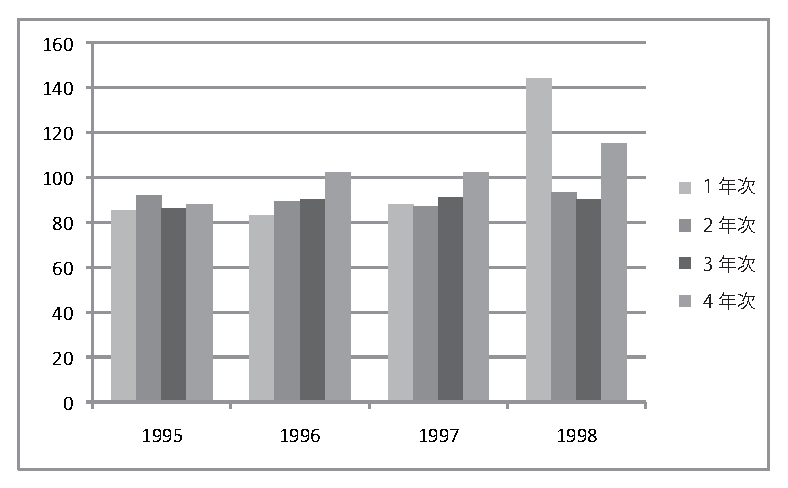
\includegraphics[width=3cm]{sample.eps}
%% 一応 OK (epsfig.sy)
% \usepackage{epsfig} % for 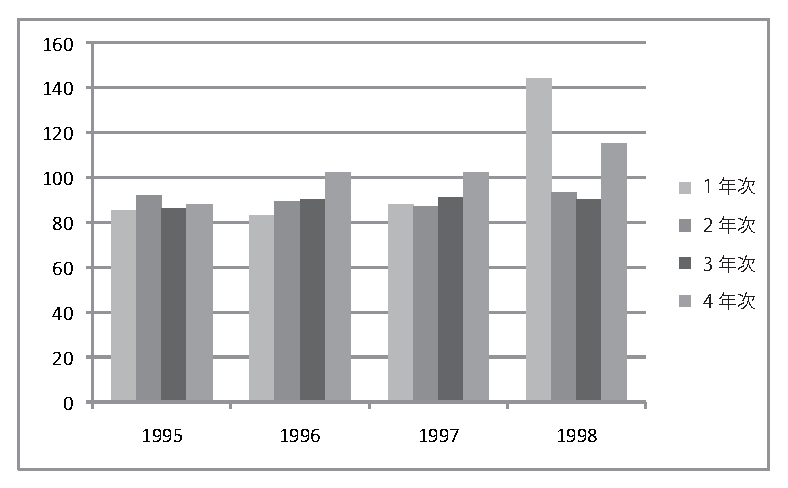
\psfig{file=sample.eps,width=3cm}
%% 以下の2つの使用はあまり勧められない (epsf.sty, epsfbox.sty)
%\usepackage{epsf} % for \epsfile{file=sample.eps,scale=0.6}
%\usepackage{epsbox} % for \epsfile{file=sample.eps,scale=0.6}

\usepackage{times} % use Times Font instead of Computer Modern

\setcounter{tocdepth}{3}	% 目次を3レベル (1.2.3) まで
\setcounter{secnumdepth}{3}	% 番号付けレベル。 3: \subsection まで 4: \subsubsection まで
\setcounter{page}{-1}

\setlength{\oddsidemargin}{0.1in}
\setlength{\evensidemargin}{0.1in} 
\setlength{\topmargin}{0in}
\setlength{\textwidth}{6in} 
%\setlength{\textheight}{10.1in}	% ページの縦幅を変更する場合には設定する
\setlength{\parskip}{0em}
\setlength{\topsep}{0em}

%% タイトル生成用パッケージ(重要)
\usepackage{mast-jp-utf8}

%% タイトル
%% 【注意】タイトルの最後に\\ を入れるとエラーになります
\title{卒業論文の書き方}
%% 著者
\author{清野 駿}
%% 指導教員
\advisor{若林 啓}

%% 年月 (提出年月)
%% 年月は必要に応じて書き替えてください。
\majorfield{ } \yearandmonth{2024年 3月}



\begin{document}
\maketitle
\thispagestyle{empty}
\newpage

\thispagestyle{empty}
\vspace*{20pt plus 1fil}
\parindent=1zw
\noindent
%%
%% 論文の概要(Abstract)
%%
\begin{center}
{\bf 概要}
\vspace{5mm}
\end{center}
わああああああああ
この文書は、筑波大学情報学群情報メディア創成学類の卒業研究論文本体のサンプルである。
このファイルを書き換えて、この例と同じような書式の論文本体を \LaTeX を使って作成することができる。

このサンプルは、学生諸君が面倒な位置決めをして表紙を作成する手間を軽減するために提供している。
もちろん、このサンプルで示す表紙は例であり、要項や手引きに 準拠していれば、
このファイルに頼らずに自分で表紙の位置決めを行ってもよい。

%%%%%
\par
\vspace{0pt plus 1fil}
\newpage

\pagenumbering{roman} % I, II, III, IV 
\tableofcontents
\listoffigures
%\listoftables		% 本ファイルでは省略してある

%% ここから本文
\pagebreak \setcounter{page}{1}
\pagenumbering{arabic} % 1,2,3


\chapter{はじめに}

研究の内容や分野によっては書き方が異なる場合もあるので、
詳しいことは指導教員に聞くとよい。
この文書は主にタイトルの作成方法と、論文の体裁を示すのみであり、
どうやったらよい論文になるかの示唆は含まれていない。

\chapter{形式}

ここでは、論文の表紙および本体の記述方法について述べる。

\section{表紙}

表紙は、{\tt $\backslash$maketitle} によって作成するため、
以下の項目に相当する文字列をそれぞれ記述する。

\begin{description} \parskip=1pt
\item{題目: }
	題目は{\tt $\backslash$title} に記述する。
	行替えを行う場合は$\backslash\backslash$ を入力する。
	ただし、題目の最後に$\backslash\backslash$ を入力するとコンパイルが通らなくなるので注意する。
	なお、4行以上の題目の場合、表紙ページがあふれるためスタイルファイル``mast-jp-xxx.sty''を変更する必要がある
	(xxx は使用文字コードに合わせて euc, sjis, utf8 のいずれかになる)。
\item{著者名: }
	著者名は{\tt $\backslash$author} に記述する。
\item{指導教員名: }
	指導教教員は{\tt $\backslash$advisor} に記述する。
\item{年月: }
	年月は{\tt $\backslash$yearandmonth} に記述する。
	\\
	年月は別途指示された場合はそれにしたがう(指示がなければ提出時のものを記述する)。
\end{description}

\section{本体}

本体は1段組で記述する。

図表には番号と説明(caption)を付け、文章中で参照する。
表 \ref{table:fundamental_data_type}と図\ref{figure:sample} は
それぞれ表と図の例である。
表の説明は上に、図の説明は下に書くことが多い。
図の挿入に用いるパッケージについては使用環境に合わせて自由に選択してほしい。

\begin{table}[hbt]
\caption{表の例}
\label{table:fundamental_data_type}
\begin{center}
\begin{tabular}{| c | r | r | r | r |}
\hline
年 度 & 1年次 & 2年次 & 3年次 & 4年次 \\
\hline
1995 & 85 & 92 & 86 & 88 \\
1996 & 83 & 89 & 90 & 102 \\
1997 & 88 & 87 & 91 & 112 \\
1998 & 144 & 93 & 90 & 115 \\
\hline 
\end{tabular}
\end{center}
\end{table}
\medskip

\begin{figure}[htbp]
\begin{center}
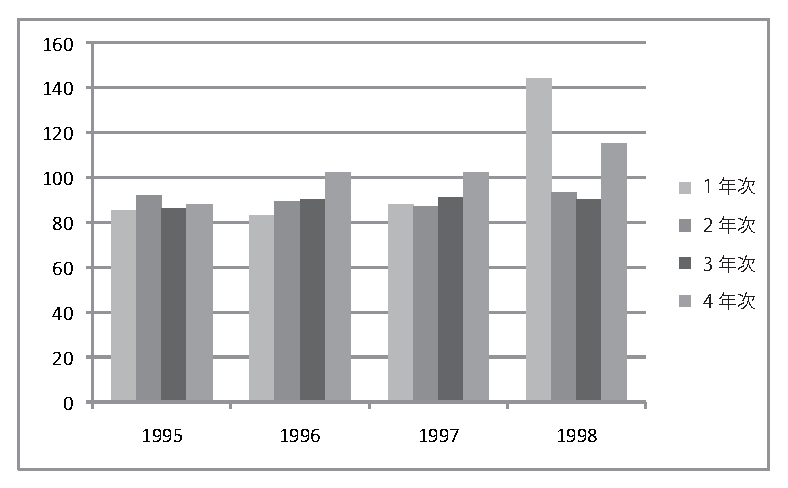
\includegraphics[scale=0.6]{sample.eps}
%% epsfig.sty を使う場合には上の行を次のように変更する
% 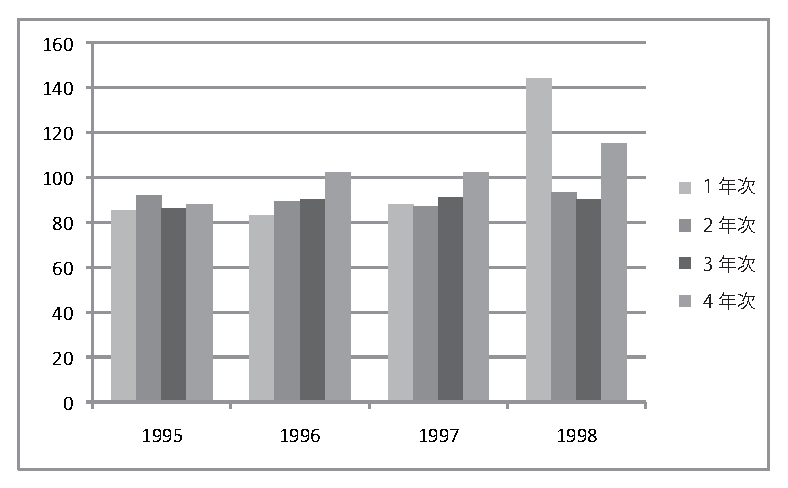
\psfig{file=sample.eps,scale=0.6}
\end{center}
\caption{図の例 (graphicx パッケージを使用)}
\label{figure:sample}
\end{figure}

詳しくは参考書\cite{okumura2010,yoshinaga2009}などを参照のこと。
奥村晴彦氏の「\TeX Wiki」 https://texwiki.texjp.org/ は
日本語の\TeX に関する情報が充実している。
具体的な文献の参照例として
本の例\cite{ware2004}、
雑誌論文の例\cite{meyer2009}、
予稿集の例\cite{hill2010}
を挙げておく。

\chapter*{謝辞}
\addcontentsline{toc}{chapter}{\numberline{}謝辞}	% 目次で左詰めするなら \numberline{} を削除する。

必須ではないが、書くことが望ましい。
\\
研究補助を受けている場合、他に指定がなければここに書く。

\newpage

\addcontentsline{toc}{chapter}{\numberline{}参考文献}	% 目次で左詰めするなら \numberline{} を削除する。
\renewcommand{\bibname}{参考文献}

%% 参考文献に jbibtex を使う場合
%\bibliographystyle{junsrt}
%\bibliography{samplebib}
%% [compile] jbibtex sample; platex sample; platex sample;

%% 参考文献を直接ファイルに含めて書く場合
\begin{thebibliography}{99}
\bibitem{okumura2010}
奥村晴彦: 
LaTeX2e美文書作成入門 改訂第5版, 
技術評論社, 2010年.	% 「年」の字はなくてもよい。

\bibitem{yoshinaga2009}
吉永徹美: 
LaTeX2$\varepsilon$辞典, 
翔泳社, 2009年.		% 「年」の字はなくてもよい。

\bibitem{ware2004} 
Colin Ware:
Information Visualization --- Perception for Design (Second Edition), 
Morgan Kaufmann Publishers, 486~pp., 2004.
%% 本のタイトルはイタリックにする流儀もある。その場合には全体を {\it ... } で囲む。
%% 氏名の途中で改行させないためには、Colin~Ware のようにハードスペースを入れる。

\bibitem{meyer2009}
Miriah Meyer and Tamara Munzner:
MizBee: A Multiscale Synteny Browser, 
{\it IEEE Transactions on Visualization and Computer Graphics},
Vol.~15, No.~6, pp.~897--904, 2009.

\bibitem{hill2010}
Emerson Murphy-Hill and Andrew P. Plack: 
An Interactive Ambient Visualization for Code Smells, 
{\it in Proceedings of the 2010 International Symposium on Software Visualization (SOFTVIS' 10)},
pp.~5--14, 2010.

\end{thebibliography}

\end{document}
